\chapter{Исследовательская часть}

В данном разделе будут приведены примеры работы программа, а также проведен сравнительный анализ алгоритмов при различных ситуациях на основе полученных данных.

\section{Технические характеристики}

Технические характеристики устройства, на котором выполнялись замеры времени представлены далее:

\begin{itemize}
	\item операционная система Windows 11 Pro Версия 22H2 (22621.674) \cite{wind};
	\item память 16 ГБ;
	\item процессор 11th Gen Intel(R) Core(TM) i5-11400 @ 2.60GГц 2.59 Ггц \cite{proc}.
\end{itemize}

При тестировании компьютер был включен в сеть электропитания. Во время тестирования устройство было нагружено только встроенными приложениями окружения, а также системой тестирования.

\section{Демонстрация работы программы}

На рисунке \ref{img:res} представлен результат работы программы. На экран выводятся результаты заемров времени для разных длин массива и разных видов сортировок в мс.
\newpage
%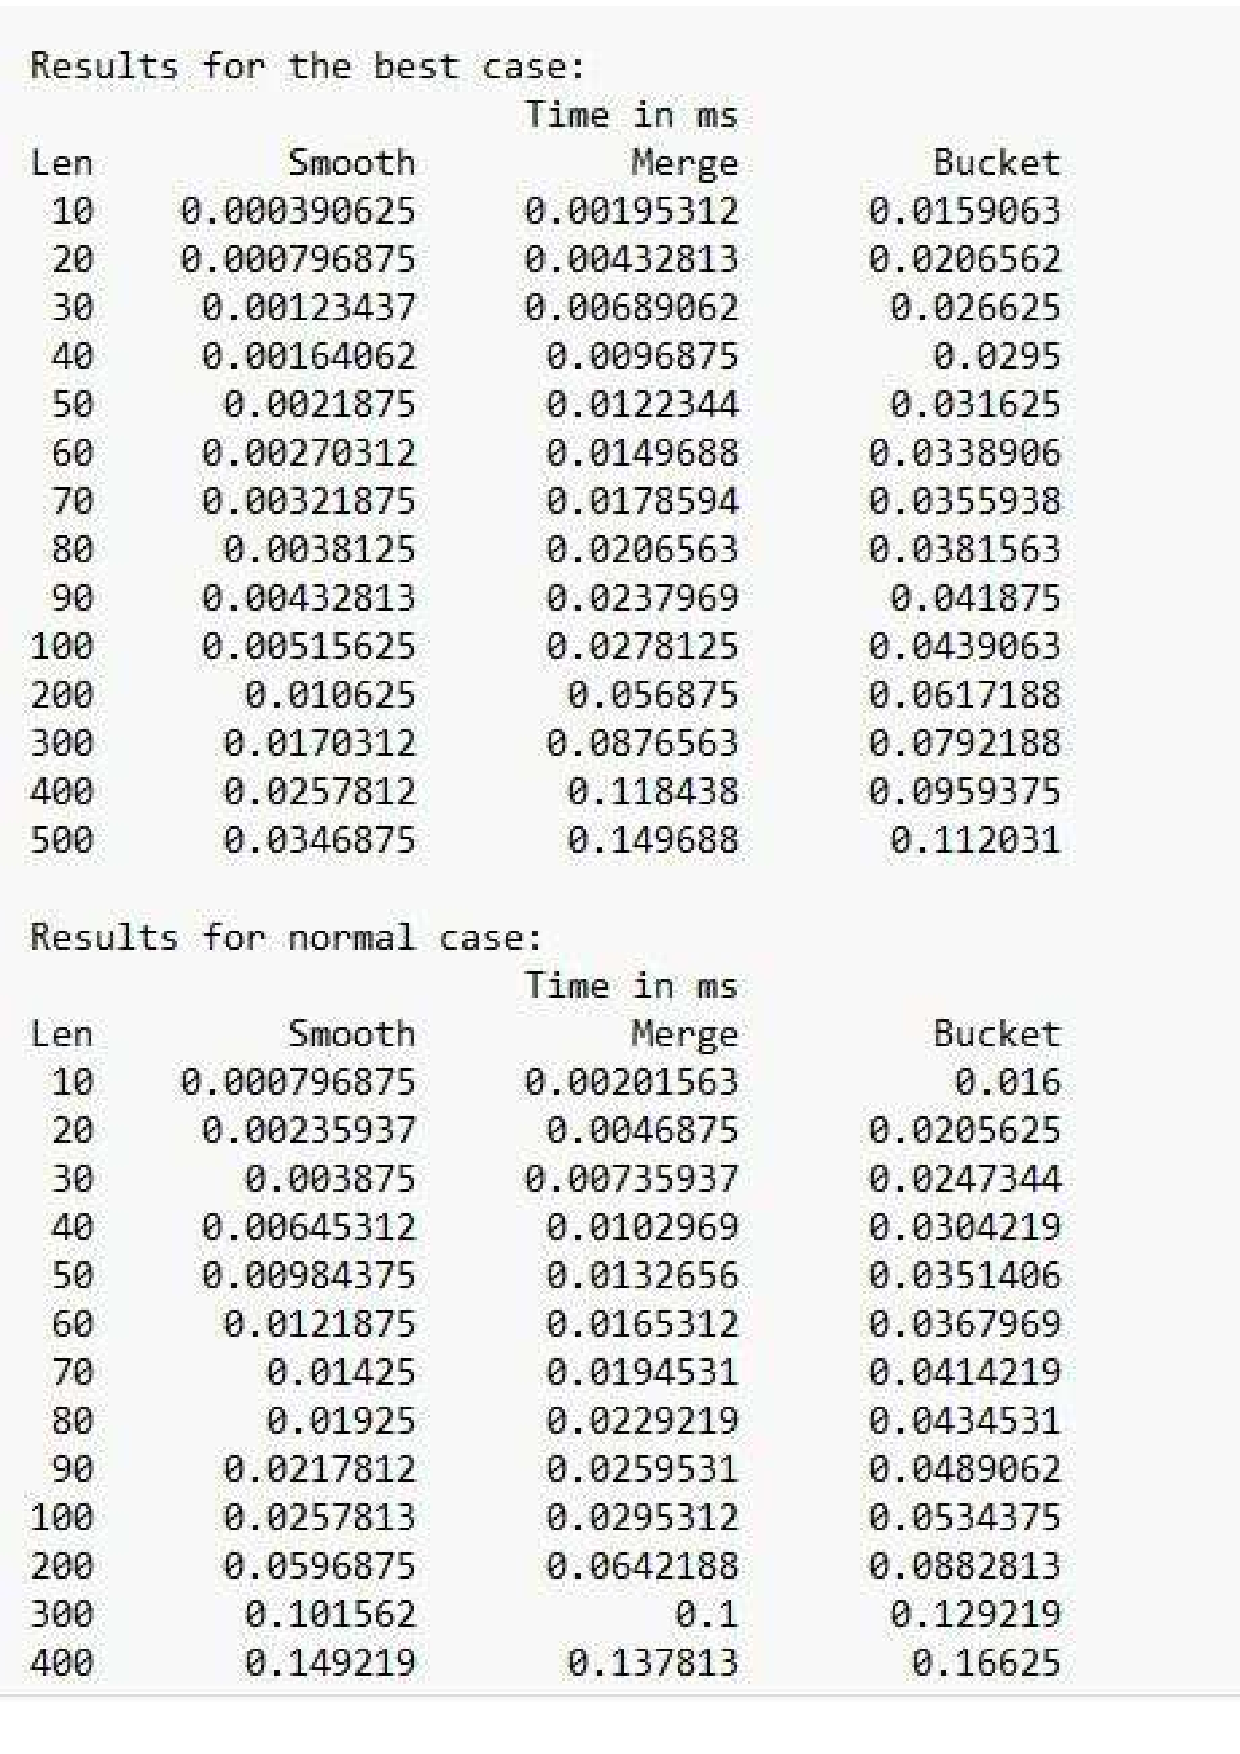
\includepdf[pages=-]{src/screen.pdf}
\begin{center}
	\centering{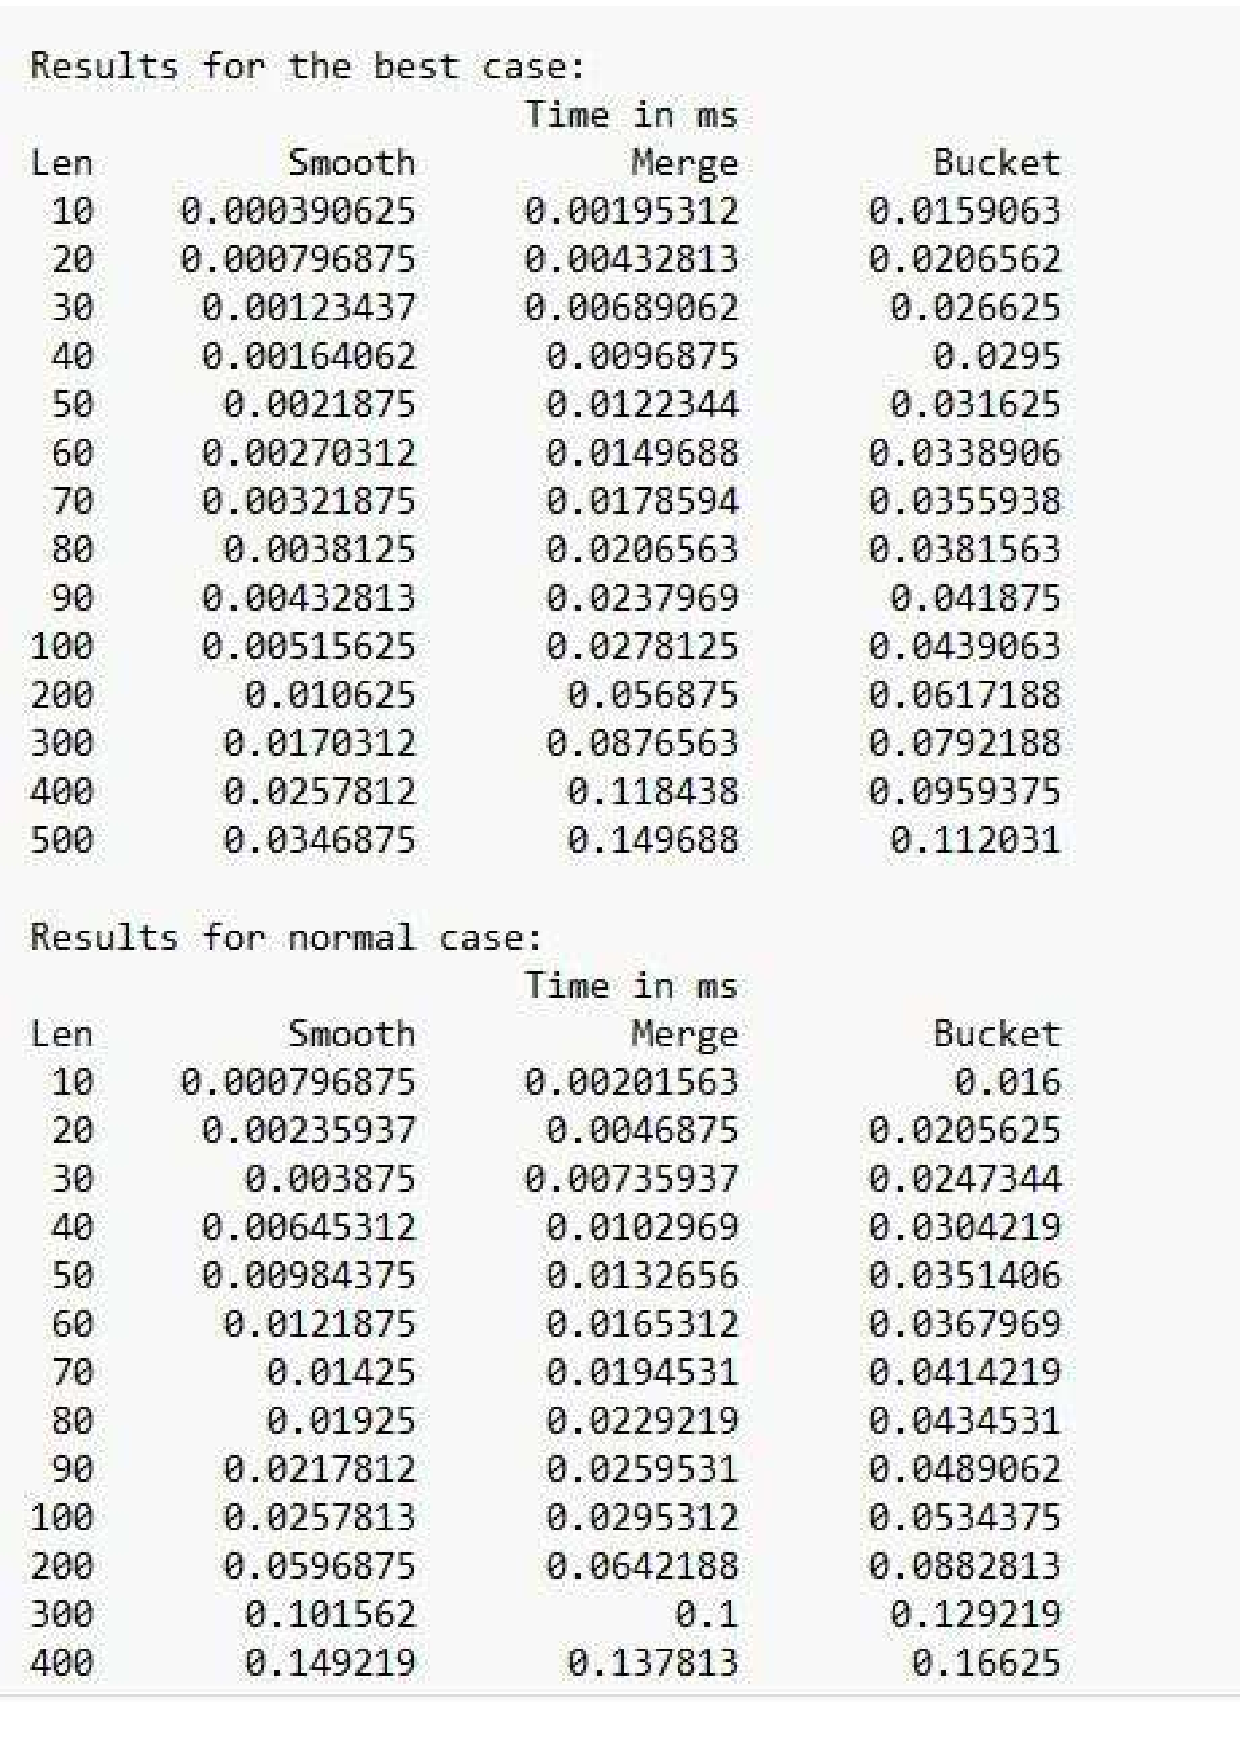
\includegraphics[trim=0 0 -20cm -21cm bb=0 0 758 461]{src/screen}}
	\captionof{figure}{Пример работы программы}
	\label{img:res}
\end{center}
\newpage
\section{Время выполнения реализаций алгоритмов}

Как было сказано выше, используется функция замера процессорного времени GetProcessTimes(...) из библиотеки Windows.h. Функция возвращает пользовательское процессорное временя типа float.

Использовать функцию приходится дважды, затем из конечного времени нужно вычесть начальное, чтобы получить результат.

\textbf{Входные данные:} целые числа от 0 до длины массива.

Результаты замеров времени работы реализаций алгоритмов сортировки на различных входных данных (в мс) приведены в таблицах \ref{tbl:best}, \ref{tbl:worth} и \ref{tbl:random}.


	\begin{center}
		\begin{threeparttable}
				\caption{Процессорное время работы реализаций алгоритмов на отсортированных данных}
			\label{tbl:best}
			\begin{tabular}{|c|c|c|c|}
				\hline
				Размер & Плавная &  Слиянием &  Блочная \\
				\hline
				100 & 0.00515625 & 0.0278125 &  0.0439063\\ 
				\hline
				200 & 0.010625 & 0.056875 & 0.0617188 \\ 
				\hline
				300 & 0.0170312 & 0.0876563 & 0.0792188 \\ 
				\hline
				400 & 0.0257812 & 0.118438 & 0.09593751 \\ 
				\hline
				500 & 0.0346875 & 0.149688 & 0.112031 \\ 
				\hline
			\end{tabular}
	
		\end{threeparttable}
	\end{center}




	\begin{center}
		\begin{threeparttable}
				\caption{Процессорное время работы реализаций алгоритмов на случайных данных}
			\label{tbl:worth}
			\begin{tabular}{|c|c|c|c|}
			\hline
			Размер & Плавная &  Слиянием &  Блочная \\
			\hline
			100 & 0.0257813 & 0.0295312 & 0.0534375\\ 
			\hline
			200 & 0.0596875 & 0.0642188 & 0.0882813 \\ 
			\hline
			300 & 0.101562 & 0.1 & 0.129219 \\ 
			\hline
			400 & 0.149219 & 0.137813 & 0.16625 \\ 
			\hline
			500 & 0.191562 & 0.177813 & 0.217812 \\ 
			\hline
			\end{tabular}
		
		\end{threeparttable}
	\end{center}




	\begin{center}
		\begin{threeparttable}
			\caption{Процессорное время работы реализаций алгоритмов на отсортированных в обратном порядке данных}
			\label{tbl:random}
			\begin{tabular}{|c|c|c|c|}
			\hline
			Размер & Плавная &  Слиянием &  Блочная \\
			\hline
			100 & 0.0259375 & 0.0267188 &  0.0546875\\ 
			\hline
			200 & 0.060625 & 0.0559375 & 0.0909375 \\ 
			\hline
			300 & 0.0960938 & 0.0876562 & 0.134844 \\ 
			\hline
			400 & 0.135313 & 0.117031 & 0.173281 \\ 
			\hline
			500 & 0.176563 & 0.147813 & 0.212031\\ 
			\hline
			\end{tabular}		
		\end{threeparttable}
	\end{center}


Также на рисунках \ref{img:graph_sorted}, \ref{img:graph_sorted_back}, \ref{img:graph_random} приведены графические результаты замеров времени работы сортировок в зависимости от размера входного массива.

\begin{center}
	\centering{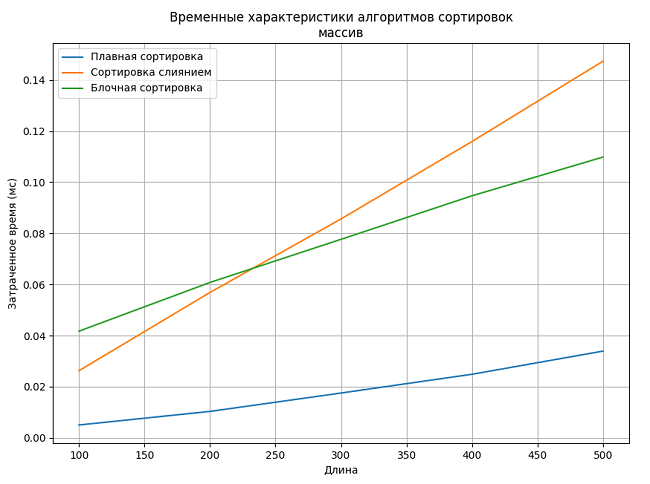
\includegraphics[trim=0 0 0 -5cm bb=0 0 484 650]{src/good}}
	\captionof{figure}{Процессорное время вычислений: упорядоченные массивы}
	\label{img:graph_sorted}
\end{center}
\newpage
\begin{center}
	\centering{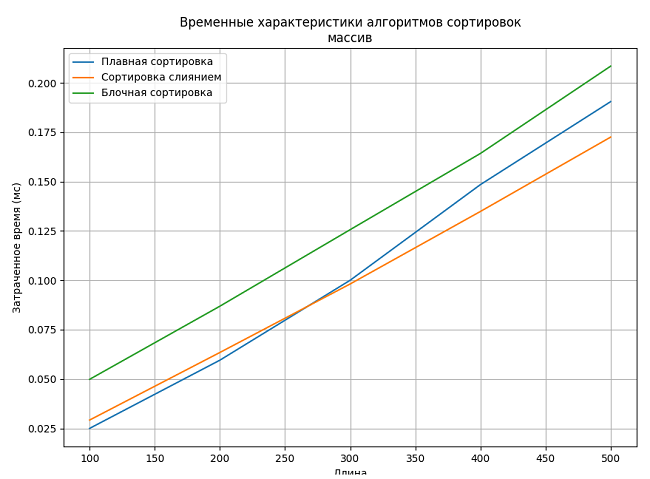
\includegraphics[trim=0 0 0 -5cm bb=0 0 484 650]{src/random}}
	\captionof{figure}{Процессорное время вычислений: массив случайных данных}
	\label{img:graph_random}
\end{center}
\newpage
\begin{center}
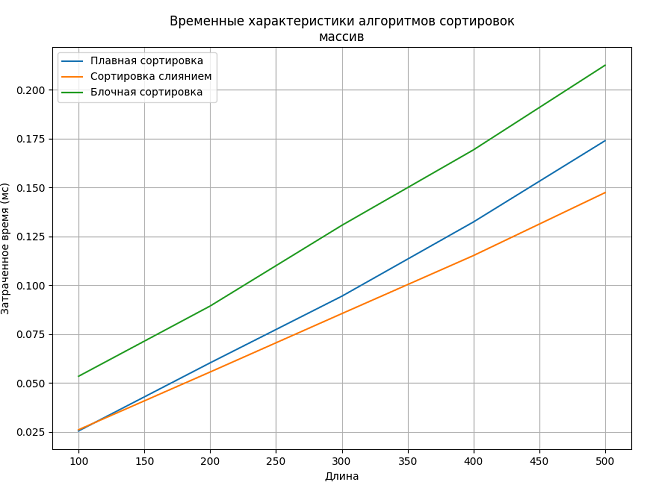
\includegraphics[trim=0 0 0 -5cm bb=0 0 484 650]{src/worst}
	\captionof{figure}{Процессорное время вычислений: обратно упорядоченные массивы}
	\label{img:graph_sorted_back}
\end{center}
\newpage


\section*{Вывод}
\addcontentsline{toc}{section}{Вывод}
Исходя из полученных результатов, на отсортированных данных плавная сортировка оказалась быстрее двух остальных. Также заметно, что зависимость процессорного времени выполнения реализации алгоритма от размера массива для данного вида упорядочивания принимает логарифмический вид при ухудшении упорядоченности входных данных. Для всех трех случаев сложность блочной сортировки подчиняется линейному закону, что говорит о том, что количество $"$корзин$"$ было выбрано оптимально.

Теоретические результаты замеров и полученные практически результаты совпадают.